\documentclass{article}
\usepackage{booktabs}
\usepackage{natbib}
\bibliographystyle{plainnat}


\usepackage{graphicx} % Required for inserting images
\usepackage{subcaption} % Required for creating figures with multiple parts (subfigures)
\usepackage{amsmath}
\usepackage{amsfonts}
\usepackage{mathtools}
\usepackage{rotating}
\usepackage{url}
\urlstyle{same}

\usepackage[skip=10pt plus1pt,]{parskip}


\DeclareMathOperator*{\argmin}{arg\,min}

\newcommand{\defeq}{\vcentcolon=}

\title{Tuneable Counterfactuals}
\author{Joshan Parmar, Pietro Lio and Soumya Banerjee}
\date{November 2023}

\begin{document}
 
\maketitle

\begin{abstract}
    By answering the question ``What must I change in the input to change the output of a model'', counterfactuals aim to explain the outputs of machine learning systems. 

    In this paper, we propose a novel methodology for generating such counterfactuals. We focus on ``sequential counterfactuals'', which give the ``changes'' as a series of ``steps'' that an end-user should take. Our ``human-in-the-loop'' methodology borrows ideas from research in Human-Computer Interaction to allow domain experts and end-users to tune the chosen counterfactuals for different use cases. 
    
    We discuss how well our methodology performs in several applications: financial (where many institutions use automated systems to decide whether individuals are entitled to loans), medical (where AI systems aid clinical professionals in decision-making) and image classification. 
    
    We exploit the ``modularity'' of our proposed method to examine possible variations on our approach and how well it performs when the model's outputs are ``noisy''. 
    
\end{abstract}

\section{Introduction}
\subsection{Explainable AI}
Automated ``artificially intelligent'' systems are increasingly intertwined with our everyday lives --- from medical diagnosis to finance and image recognition. While some situations will use directly interpretable models --- such as logistics regression \citep{molnar_interpretable_2023}
--- others will be ``black-box'' \citep{castelvecchi_can_2016}. 
For consumers to trust these ``black-box'' models, they often want some ``explanation'' as to what this automated system is doing --- an answer to why it made the decision it did. Explainable AI (XAI) is a field of research that aims to develop tools and techniques to answer these questions. XAI can also be used for debugging models by finding where the model has learnt spurious relationships in the training data and providing algorithmic accountability.

\subsection{Counterfactuals}
One way of providing these explanations is through counterfactuals. The classic example of a counterfactual explanation of a model involves a situation where we have trained a model to decide whether a bank should provide an individual with a loan. A helpful way to explain the predictions this model makes is to say what a user must modify to change the prediction made by a model. For example, ``You were denied this loan, but if your income was £10,000 higher, you would have been granted this loan'', or ``You were granted this loan, but you would not have been granted a loan of a higher value''. Similarly, we could say ``This image was classified as a \(1\), but if we filled in these pixels, the image would be classified as a \(0\).''

Formally, given a data point \(x\) and a classification model \(f\), we define a counterfactual as a different data point \(x'\) such that \(f(x) \neq f(x')\). We want our counterfactual point to be, by some metric, close to the original point, so we can solve this through an optimization problem.

\subsubsection{Existing methodologies for Generating Counterfactuals}
To examine the effectiveness and utility of this novel methodology, we compare it against some existing methodologies for generating counterfactuals. While we give a broader overview of the current research in our Literature Review, we begin by giving a detailed mathematical explanation of our two choices of comparisons. We chose these options as there are publicly available Python packages \citep{van_rossum_python_1995, klaise_alibi_2021} implementing these. As we also make a Python implementation of our methodology publicly available, these are reasonable points of comparison --- though it is not exhaustive. 

AlibiExplain, developed by~\cite{klaise_alibi_2021} implements the method described by~\cite{wachter_counterfactual_2017}. 
This methodology works by performing the following minimization:
\begin{equation}
    \argmin_{{x'}} 
    \left(
        \max_{{\lambda}} \left(
            \lambda 
            \left(
                f_{w} \left({x'}\right) - y_i
            \right)^2 % chktex 3
            +
            d 
            \left(
               x_i, {x'}
            \right)
        \right)
    \right)
\end{equation}
In this case, \(\left(x_i,y_i\right)\) represents the point we are trying to find a counterfactual for, \(f_w\) is the model and \(d\) is some distance metric. Wachter et al.\ propose using the ADAM distance metric \citep{kingma_adam_2017}. 

Klaise et al.\ also implement a more complex methodology that utilizes ``prototypes'', as introduced by~\cite{van_looveren_conditional_2021}.
This methodology also minimizes a loss function \(\mathcal{L}\) over some \(D\)-dimensional feature space. The loss function they use is 
\begin{equation}
    \mathcal{L}=c \cdot L_{pred}+ \beta\cdot L_1+L_2+L_{AE}^\gamma+L_{proto}^\theta
\end{equation}
\begin{equation}
    L_{pred} = 
    \max \left( 
        \underbrace{
            \left[
                f(x_0 + \delta)
            \right]_i % chktex 3
        }_{
            \text{Original class}
        }  - \underbrace{
            \max_{t\neq i} \left(
                \left[
                    f(x_0 + \delta)
                \right]_i % chktex 3
            \right)
        }_{
            \text{New class}
        },
        -\kappa
    \right)
\end{equation}
\(L_\text{pred}\) encourages the class to change, \(L_{AE}^\gamma\) penalizes (by a factor of \(\gamma\)) out of distribution counterfactual instances (by using the \(L_2\) reconstruction error from an auto-encoder\footnote{An Auto-encoder is a neural network trained to copy its input to its output. The hidden layer acts as a bottleneck in a lower-dimensional space. It can be, in some senses, be considered a compression algorithm designed to work well on the distribution in the training set.} \citep{jordan_introduction_2018} 
trained on the training set), \(L_{proto}\) acts by a factor of \(\theta\) to both speed up the search process and guide the perturbation towards an interpretable counterfactual, and \(L_1\) and \(L_2\) correspond to the usual norms.
Mathematically, \(L_{proto}\) works by first using an auto-encoder \(\text{Enc}:\mathbb{R}^N\rightarrow \mathbb{R}^E\) to project \(x\) onto an \(E\)-dimensional latent space \(\mathbb{R}^E\). Then, for each class, \(i\), they apply this encoder to all training set instances belonging to that class. Then take the 
\(k
\)-nearest instances in this latent space and define:
\begin{equation}
    \text{proto}_i \defeq \frac{1}{k}  \sum_{t=1}^k ENC(x_t^i)
\end{equation}
and \(j\) as the ``closest'' other class in \(\mathbb{R}^E\) latent-space., 
\begin{equation}
    j = \argmin_{i\neq \text{original}}  \left| ENC \left( x_0 \right)- \text{proto}_i \right|_2
\end{equation}
Finally, the prototype loss term is defined as the distance of the proposed counterfactual to the average representation of the new class in \(\mathbb{R}^E\) latent space.
\begin{equation}
    L_{\text{proto}}  = \theta \cdot \left| ENC\left(x_0  + \delta \right) - \text{proto}_j \right| _2^2
\end{equation}
In effect, this guides perturbations towards the ``nearest prototype''.
We do not provide a specific encoder, so class representations are built using k-d trees \citep{bentley_multidimensional_1975}. 



\subsubsection{Practical uses of Counterfactual Explanations~\label{sectoin:practical_uses}}
As with all forms of explanation for automated systems, they can increase a user's trust in an automated system \citep{inam_explainable_2021}. 
By attempting to approximate the ``reasoning'' that these automated systems have employed, users can assess whether they agree with this reasoning. These counterfactual explanations can also be tuned to be actionable --- this means that an end user can take actions based on their received explanations. For example, if an explainer suggests that an applicant was denied for a loan but would have been accepted for a smaller loan, the applicant can respond by applying for this smaller loan. Similarly, in a medical situation, if the explainer suggests that a patient who exercised more would be less likely to have severe complications from a disease, the patient could respond by doing this. Of course, not all changes are possible for all situations, so a ``tuneable'', ``human-in-the-loop'' methodology is beneficial.

Similarly, as discussed by~\cite{blackwell_bias_2022}, users of an automated system are entitled to an explanation of why such a system made the decision it did. Counterfactual explanations can be one part of meeting this legal requirement \citep{goodman_european_2017}. 
Counterfactuals can also help data scientists understand the model's internal structure better and correct for unintentional biases in the training data. For example, suppose counterfactuals generated for a financial model suggest that ``protected characteristics'' should be changed to change the output of the model. In that case, it is likely that the model has learnt unintended biases and that further work is needed to de-bias the training data before deploying the model in practice. 

When domain experts are presented with such ``counterintuitive'' explanations, they can be prompted to examine the training data set for these biases, leading to fairer, more accurate models. Ultimately, this also can be a part of legal requirements to conduct impact assessments for model's ``bias [and] effectiveness'' \citep{office_of_ron_wyden_algorithmic_2022}.


\section{Methods}

\subsection{Methodology for Generating Counterfactuals}
We can summarize our general methodology as ``chaining together'' simple local models to find counterfactual explanations in a highly tuneable way.

We begin by fitting simple surrogate models (Section~\ref{section:surrogate_models}) to the variation of each relevant feature in the model. We then use a tuneable set of scoring rules, as discussed in Section~\ref{section:scoring_rules}, to assign each of these a score. If any of these models suggest changing that variable is sufficient to cross the decision boundary, we return the ``best'' such model (in terms of this score). Otherwise, we are able to iterate from the the extrema points of these model (the feature value that takes us closest to crossing the decision boundary). Various strategies are possible to implement this ``iterative search'', which we discuss in detail in Section~\ref{section:search}.


\subsubsection{Surrogate Models\label{section:surrogate_models}}
These surrogate models, which we will often refer to as single variable explainers (SVEs), attempt to explain the dependence of the model's output on the variation of one parameter locally. 

For a particular variable, we generate a set of input data points by replacing that variable with other values that the variable takes in the training data set. Either we do this through Monte-Carlo-esque sampling --- i.e.\ replacing with randomly chosen other values in the data set --- or by selecting uniformly placed points across some interval, such as \(\left[\mu \pm \sigma \right]\) (where \(\mu\) is the variable's mean value in the training data and \(\sigma\) is the standard deviation) or defined ``quantiles'' of the values of that feature in the training data. We then apply the (black-box) model to these to get a series of sampling variables and class probabilities pairs. 

We then fit a simple (explainable) model to this new data set. We usually use either a Gaussian Process or sometimes a linear model. Our code is sufficiently general to allow for any SciKit-Learn regression model to be used. 

\subsubsection{Scoring Rules\label{section:scoring_rules}}
A range of rules can be used to score these models, by default, we consider the following:

\begin{equation}
    S_\text{basic}(x_i^\text{new}) = \text{abs}\left( \text{Underlying Model}\left(\mathbf{x^\text{original}}\right) - \text{SVE}\left(x_i\right) \right) 
    \label{equation:sve_score_basic}
\end{equation}

In some cases, our model to recommend smaller changes to features so we can also consider the following:

\begin{equation}
    S_\text{masked}(x_i^\text{new}) = \exp \left( -\frac{1}{2}\left(\frac{ x_i^\text{new} - x_i^\text{original} }{\sigma^\text{training}_i \times f(w_i)} \right)^2\right) \times S_\text{basic}(x_i^\text{new}) % chktex 3
    \label{equation:sve_score_masked}
\end{equation}

Finally, each score is weighted by a user-provided ``feature changeability score'' that quantifies how easily a feature can be changed. \(S_{\text{Final}}\left(x_i^{\text{new}}\right) = w_i \cdot S\left(x_i^{\text{new}}\right) \) Borrowing ideas from the field of ``Human Computer Interaction'', this allows the user to ``tune'' the methodology to their use case.

This is visualized in Figure~\ref{figure:scoring_example}.

\begin{figure}[t]
    \centering
    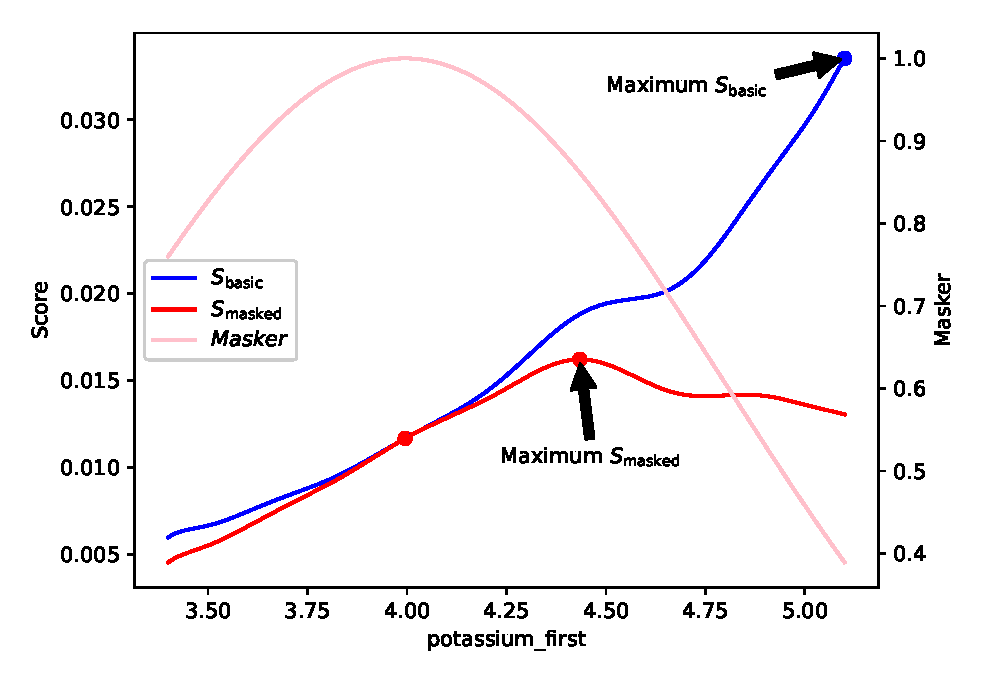
\includegraphics[width=\linewidth]{figures/scoring.eps}
    \caption{Example of how scoring rules work. The ``basic'' scoring rule is shown in blue, while the ``masked'' scoring rule is shown in red. The ``masked'' scoring rule is ``masked'' by a bell curve, shown in pink.\label{figure:scoring_example}}
\end{figure}

\subsubsection{Search Rules~\label{section:search}}
Our search system can be considered a modified form of ``depth-first'' search.
We initially train surrogate models for each ``changeable'' feature of the example. We select the best (using the rules described in Section~\ref{section:scoring_rules}) and ``change'' that feature to the value that takes us closest to it's best value. From this new point, we retrain surrogate models and repeat this process until we cross our decision boundary. If we ``run out'' of features to change, we return one layer up the ``tree'' and change the next best feature. We continue this process until we cross the decision boundary. This process is illustrated in Figure~\ref{figure:search_example}.

We note that we have built our system such that it is ``modular'', so that we can easily change the search process. For example, we can change the order in which we change features. We can also change the ``stopping criteria'' --- i.e.\ when we stop changing features and decide there does not exist a counterfactual subject to the given criteria. 

In terms of technical implementation, this requires the definition of a simple ``searcher'' class that can be passed to our ``counterfactual'' class. This searcher class only requires two functions. Firstly, {\verb|get_next_evaluation_set|} should, given the current ``node'', select which nodes to evaluate next. Similarly, {\verb|get_next_node|} should, given the scores of the previous evaluation, select the next node to evaluate. This allows for a wide range of search strategies to be implemented. 

For this paper we use only \(S_\text{basic}\), as defined in Equation~\ref{equation:sve_score_basic}.

\begin{sidewaysfigure}
    \centering
    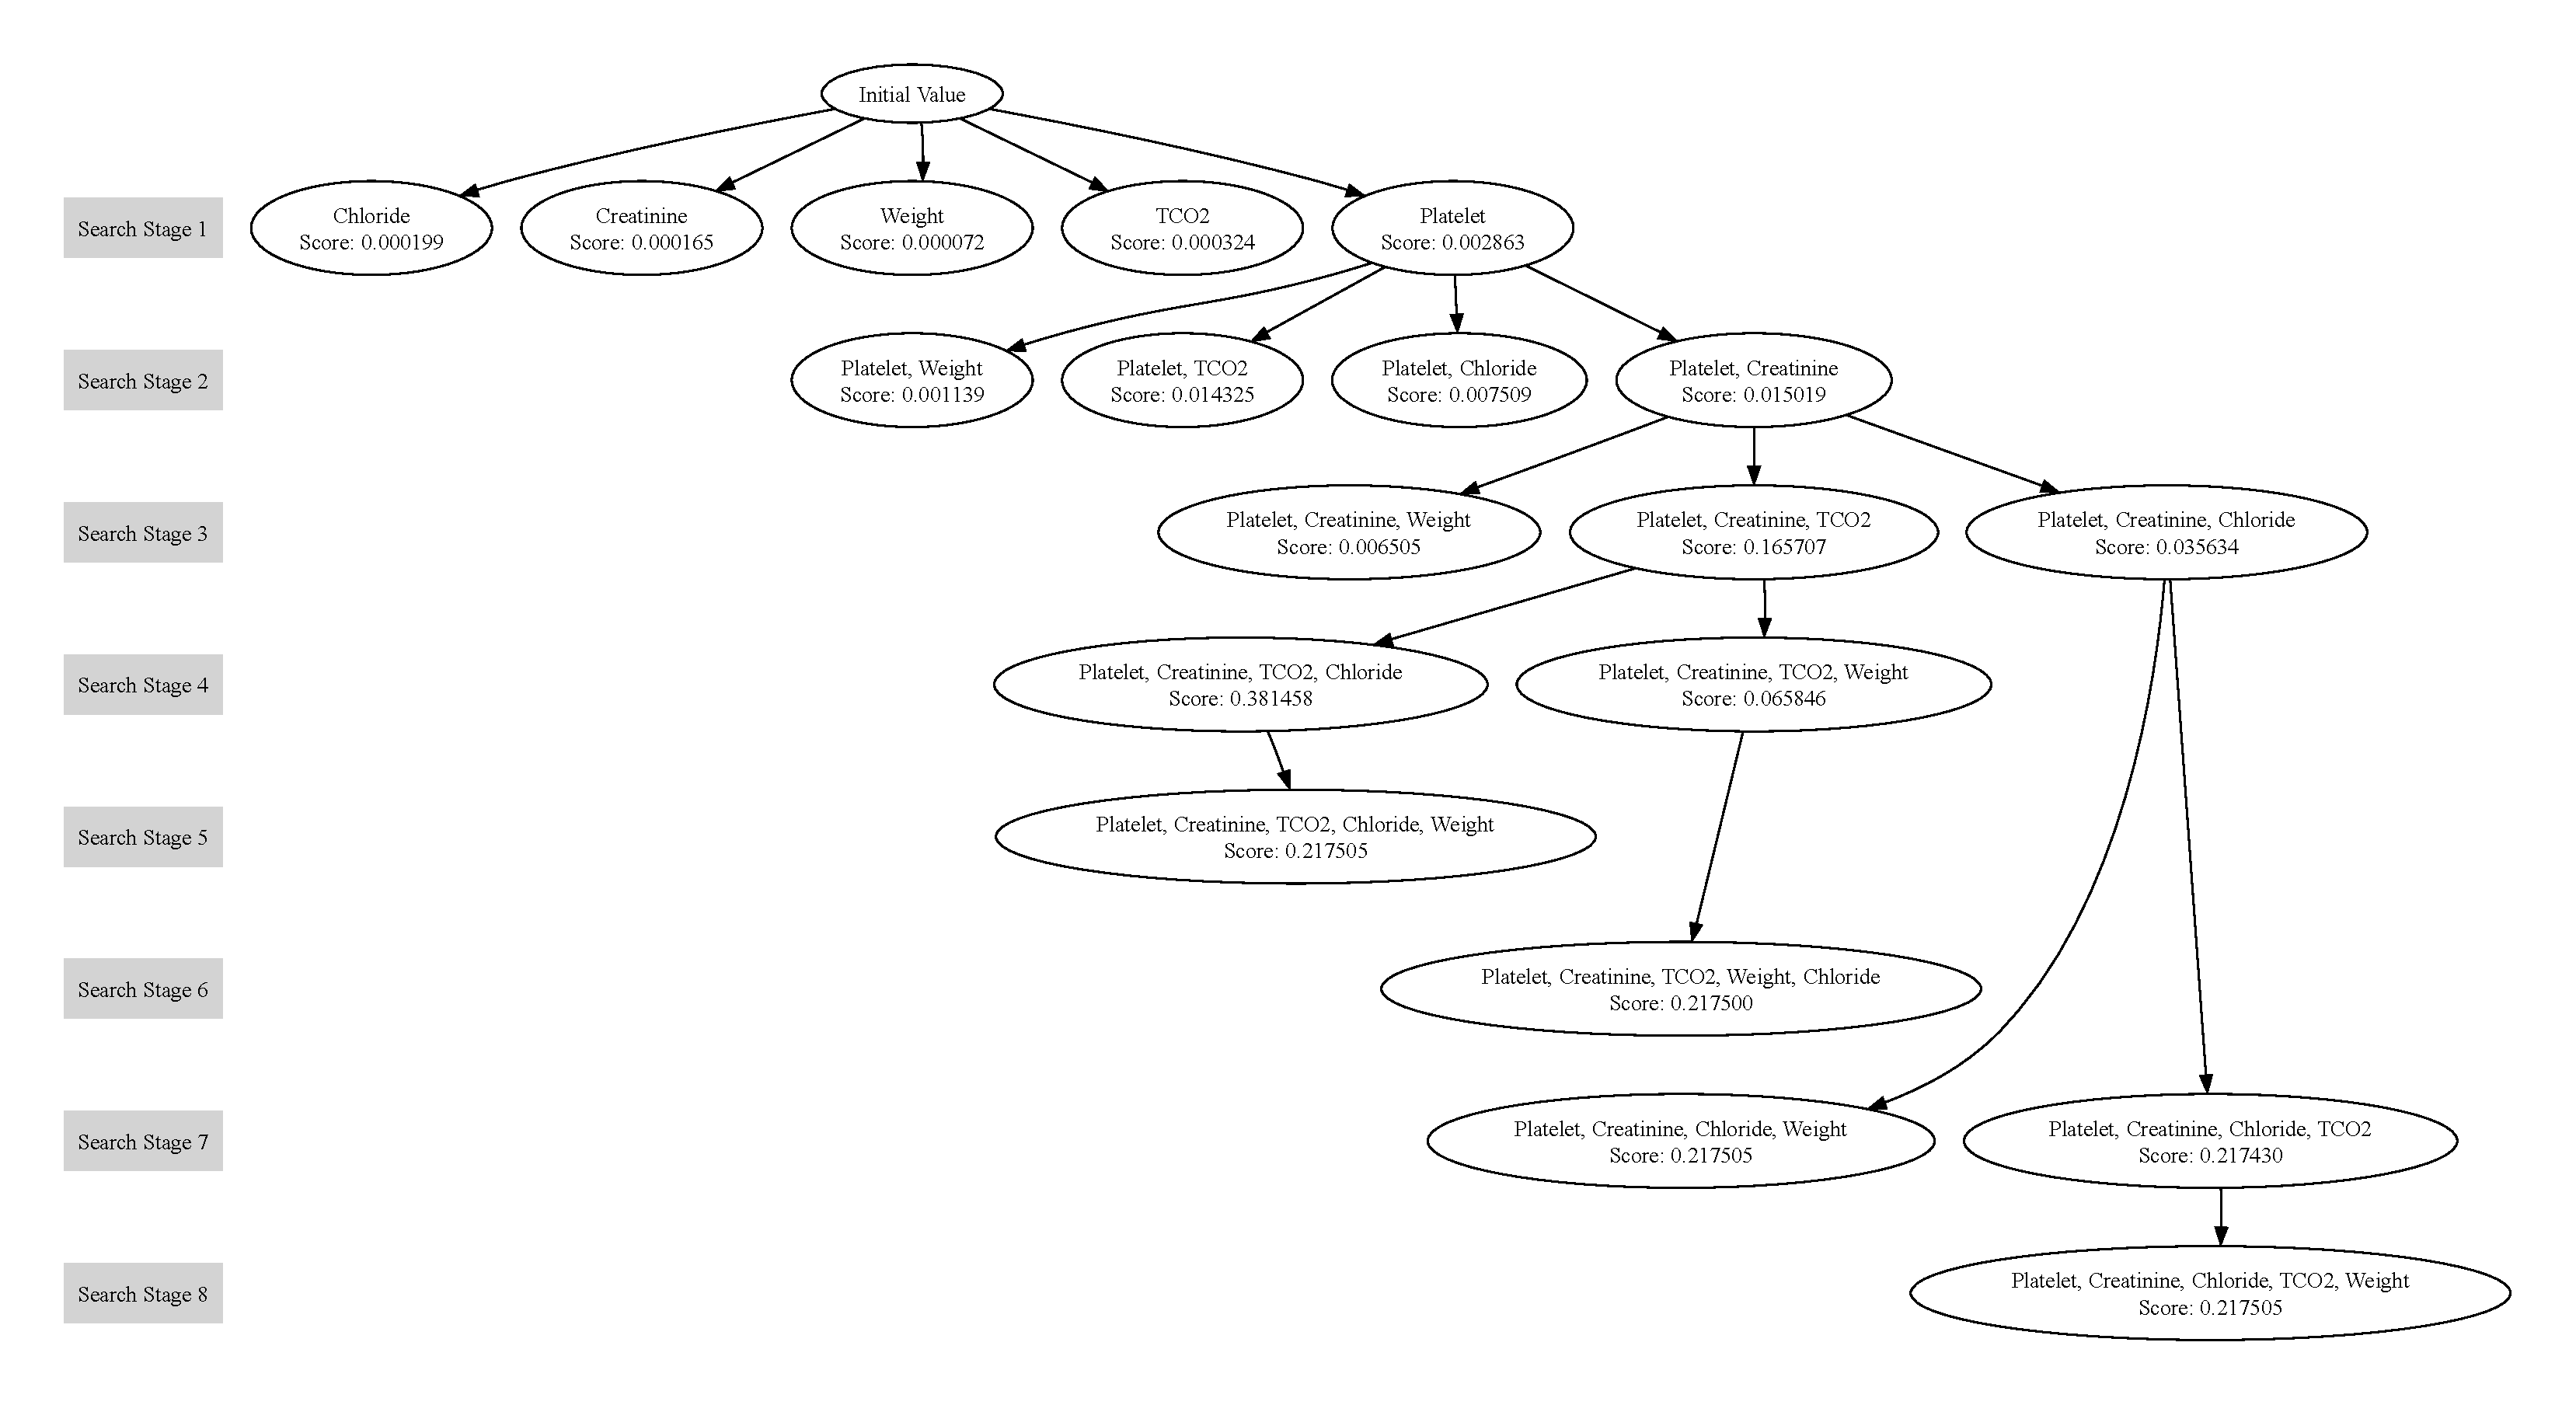
\includegraphics[width=\linewidth]{figures/round-table.gv.pdf}
    \caption{Example of the default search process we have implemented.\label{figure:search_example}}
\end{sidewaysfigure}

\subsection{Evaluation Methodology}
We will evaluate our method by training simple models on simple data-sets and evaluating how the counterfactuals generated by our model compare to those generated by some existing methodologies for generating counterfactuals. While this is not an exhaustive comparison, we have chosen some methodologies with existing publicly available implementations as valuable points of comparison. As our framework is available as an easily installable Python package, this accurately compares what other options domain experts will have at their disposal to explain machine learning models. We will use qualitative and quantitative metrics to evaluate our counterfactuals compared to those generated by other models. 


\subsubsection{Evaluation Metrics\label{section:evaluation_metrics}}
In terms of quantitative metrics, we first examine speed. An ideal algorithm to generate counterfactuals will be able to generate them quickly. Of course, this is not a perfect metric --- as different technical implementations of the algorithm will lead to different run times. Similarly, different hardware may allow the algorithm to perform at different speeds. However, studying this gives us a rough estimate of the algorithm's efficiency. We conducted all our experiments on a 2022 M2 MacBook Pro with 24 GB of RAM. %chktex 13

Additionally, as we want our counterfactual to be ``close'' to the original data point, we compare the distance to the original data point in terms of both the \(L_1\) and \(L_2\) norms. For these distance metrics, we normalize them relative to the variation of that feature present in the training data. We define the standardized \(L_k\) distances as:   
\begin{equation}
    L_k^{\text{Standardized}} = \sqrt[k]{\sum_{i=1}^N \left(\left( \frac{\left|x^{\text{new}}_i - x^{\text{old}}_i \right|}{\sigma_i^\text{Training Set}}\right)^k\right)} % chktex 3
\end{equation}
Similarly, we want our counterfactuals to change as few features as possible, so we also compare the number of feature changes. Furthermore, we often want our counterfactual to be ``plausible'' --- coming from a distribution similar to the original training data set --- so we shall also measure the standardized \(L_2\) distance to the nearest training data point.

Some of our qualitative metrics will include the ones used by~\cite{schut_generating_2021}
. We want our counterfactuals to be both ``unambiguous'' and ``realistic''. However, we also want them to reflect the model accurately. We also qualitatively examine what we ``learn'' about the model from the counterfactuals, and how ``useful'' such a counterfactual may be to a user.

\subsubsection{Evaluation Data-sets}
As we discussed in Section~\ref{sectoin:practical_uses}, these counterfactual explanations can be useful in financial and medical situations, so we evaluate our methodology on these. Since our methodology can be easily visualized on image datasets, we also evaluate it on this.

% \paragraph{Financial Data-set}Our first evaluation uses a ``simulated'' data set %\citep{noauthor_credit_nodate}. 
% We made this decision due to the lack of publicly available data sets for which appropriate documentation of their data collection methods exists. Since this project aims to evaluate the methodology for explaining models rather than the models themselves, using a simulated data set is unlikely to affect our results significantly. 

% This data set contains 12 features (Age, Annual Income, Home-ownership, Employment length (in years), Loan intent, Loan grade, Loan amount, Interest rate, Loan status, Percent income, Historical default and Credit history length) and 32581 examples.
% This data set contains only a small amount of missing data: 3116 loans were missing interest rate data, and 895 were missing employment rate information. For this reason, we chose to remove these 3943 data points. 

\paragraph{MIMIC}
The MIMIC (Multi-parameter Intelligent Monitoring in Intensive Care) II data set \citep{saeed_mimic-ii_2011}
contains physiological signals and vital signs time series captured from patient monitors, along with comprehensive clinical data for tens of thousands of Intensive Care Unit (ICU) patients. 
We use a ``pre-processed'', smaller version of this data set produced by~\cite{raffa_clinical_2016}
, which contains information about the patient, such as age, gender, weight and BMI, information as to if and when the patient entered ICU, information about the patient's clinical and medical history. 

\paragraph{MNIST}
The MNIST data set is a large data set of labelled handwritten digits. It contains 70000 individually labelled 28 by 28 images with pixel values being integers from 0 to 255. This handwritten digit data set is standard across research in this field~\cite{verma_counterfactual_2022}
, presenting a valuable point of comparison. 

\subsubsection{Training the simple models}
For the medical datasets, we train ``Multi-layer Perceptron'' (MLP) Classifiers\footnote{
A multi-layer perceptron is a supervised learning algorithm made up of a feed-forward neural network with three types of layers --- input, hidden and output. These layers are usually fully connected. Each layer is usually followed by some non-linear activation function to allow the method to model non-linear relationships.
} with two hidden layers of size \(20\) to evaluate our explanation methodology on. We select a subset of useful columns in the dataset for this purpose.

Similarly, for our image dataset, we use a MLP with hidden layers of size 100 and 200.

% \subsection{Further Evaluations}
% \subsubsection{Choice of Scoring Function}
% For our MIMIC dataset, we will also compare the results we generate using the various scoring functions defined in Equations~\ref{equation:sve_score_basic} and~\ref{equation:sve_score_masked}.


\section{Results and Discussion}
\subsection{Medical Data-set}
By running our methodology using ``gaussian process'' surrogate models, we can example how our proposed method works on medical data. Consider the patient described in Table~\ref{table:mimic_patient}. Figure~\ref{figure:mimic_counterfactuals} shows the counterfactuals generated by our methodology. These counterfactuals are ``plausible'', i.e.\ taking ``realistic'' values for the variables present\footnote{We discuss possible correlation within the variables making this not ``realistic'' in our Future Work section.}. They are also ``unambiguous'' --- they clearly show a change in classification, increasing the probability of death from \(0.0\) to \(0.99\). 

This presentation of our results highlights a key benefit of our methodology, that it creates ``sequential'' counterfactuals. This means that it gives a series of ``steps'' that a user can take to change the model's output. This is particularly useful in medical situations, as these can often be actionable where a user can take these steps to improve the patient's health. We can use changeability scores to ``tailor'' our results here, by assigning higher scores to the features we want to change. For example, we can assign a higher score to the ``weight'' feature, as this is something that is easier to change than the ``age'' feature. As these scores would be different for each patient, our method allows for a domain expert to tune this ``human-in-the-loop'' methodology.

\begin{table}[]
    \centering
    \begin{tabular}{@{}ll@{}}
    \toprule
    \textbf{Feature}      & \textbf{Value}    \\ \midrule
    age                   & 71.317250         \\
    bmi                   & 28.058252         \\
    weight\_first         & 43.600000         \\
    icu\_los\_day         & 1.910000          \\
    hospital\_los\_day    & 22.000000         \\
    day\_icu\_intime\_num & 7.000000          \\
    hour\_icu\_intime     & 5.000000          \\
    map\_1st              & 87.000000         \\
    hr\_1st               & 71.000000         \\
    temp\_1st             & 97.400002         \\
    spo2\_1st             & 100.000000        \\
    abg\_count            & 2.000000          \\
    wbc\_first            & 7.200000          \\
    hgb\_first            & 11.700000         \\
    platelet\_first       & 209.000000        \\
    sodium\_first         & 139.000000        \\
    potassium\_first      & 2.900000          \\
    tco2\_first           & 26.000000         \\
    chloride\_first       & 101.000000        \\
    bun\_first            & 6.000000          \\
    creatinine\_first     & 1.000000          \\ \midrule
    \textbf{day\_28\_flg} & \textbf{0.000000} \\ \bottomrule
    \end{tabular}
    \caption{(Processed) MIMIC Patient data for a patient who did not die within 28 days of entering ICU.\label{table:mimic_patient}}
\end{table}

\begin{figure}
    \centering
    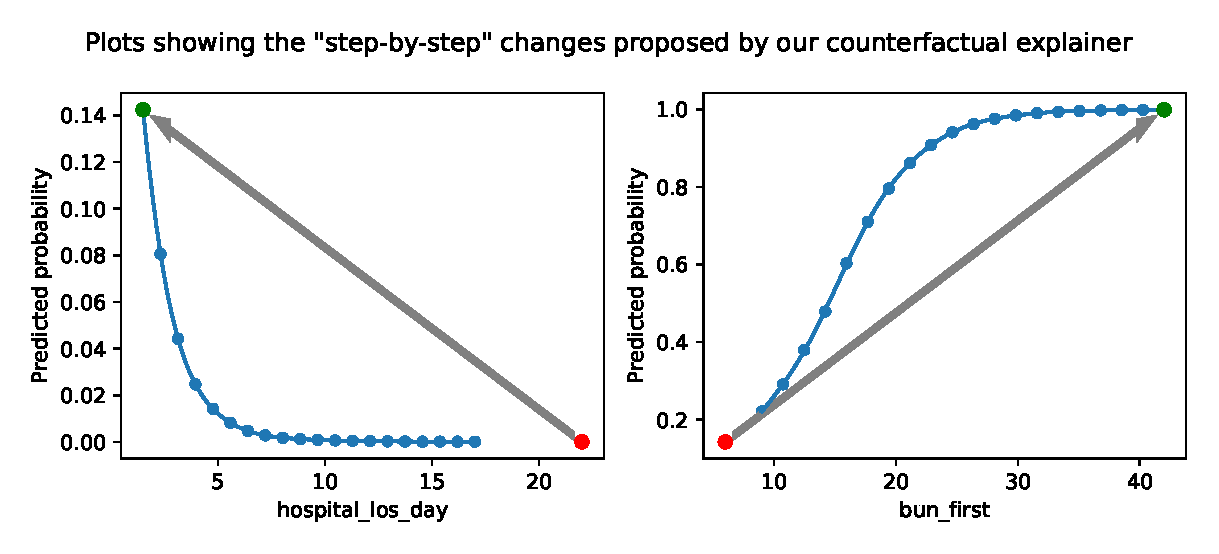
\includegraphics[width=\linewidth]{figures/mimic_counterfactual_example.eps}
    \caption{Example counterfactual generated with our proposed methodology. Each image shows one of the ``steps'' suggested by our methodology.\label{figure:mimic_counterfactuals}}
\end{figure}

\subsection{Image Data-set}
By running our methodology with ``linear'' surrogate models, and allowing features to take values between the \(10\%\) and \(90\%\) quantiles of the training data, we can generate counterfactuals for the MNIST data set. We can see some examples of these in Figure~\ref{figure:mnist_counterfactuals}.

\begin{figure}
    \centering
    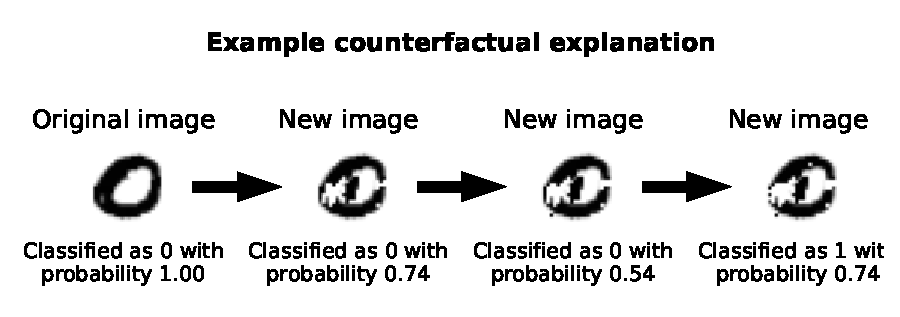
\includegraphics[width=\linewidth]{figures/mnist_counterfactual_example.eps}
    \caption{Example Example counterfactual generated with our proposed methodology. The first picture shows the original image, with the final showing the counterfactual. The middle images show some of the ``steps'' taken to get from the original image to the counterfactual.\label{figure:mnist_counterfactuals}}
\end{figure}

These counterfactuals are giving us an insight into how the model is making its classification decisions. In some sense it begins to ``fill-in'' the \(0\) to make it look more like a \(1\). 

Similarly, running the previously described existing methodologies on this example, lead to different, almost ``advserarial'' counterfactuals. These are shown in Figure~\ref{figure:mnist_counterfactuals_other}\footnote{These were also generated with ``quantile'' feature bounds, but rather using \(5\%\) and \(95\%\) bounds as theses methods were unable to find any counterfactuals in the \(10\%-95\%\) range.}.

\begin{figure}
    \centering
    \begin{subfigure}{\linewidth}
        \centering
        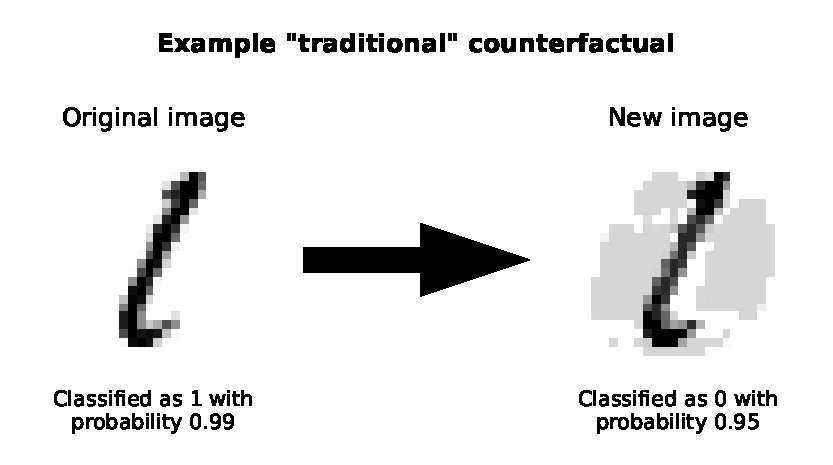
\includegraphics[width=\linewidth]{figures/mnist_counterfactual_trad_example.eps}
        \subcaption{Example counterfactual generated with the methodology of~\cite{wachter_counterfactual_2017}\label{subfigure:mnist_counterfactual_trad_example}}
    \end{subfigure}
    \begin{subfigure}{\linewidth}
        \centering
        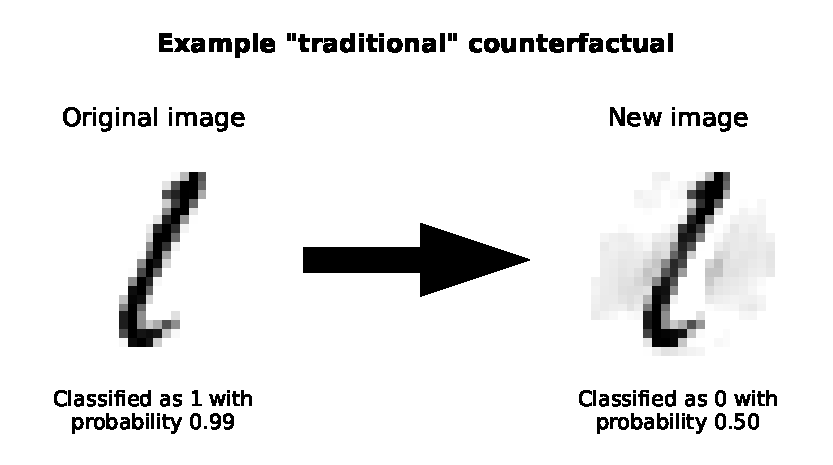
\includegraphics[width=\linewidth]{figures/mnist_counterfactual_proto_example.eps}
        \subcaption{Example counterfactual generated with the methodology of~\cite{van_looveren_conditional_2021}\label{subfigure:mnist_counterfactual_proto_example}}
    \end{subfigure}
    \caption{Example counterfactuals generated with other methodologies. The first picture shows the original image, with the final showing the counterfactual.\label{figure:mnist_counterfactuals_other}}
\end{figure}

We can see a clear qualitative difference in types of counterfactual generated between our methodology and the two ``comparison'' methods. In a sense, our method works more to ``transform'' the image from a \(0\) into a \(1\), while the other methods work to ``perturb'' the image from a \(0\) into a \(1\). Since our method ``chains together'' single pixel changes, there is an ``inbuilt'' incentive for our method to change fewer pixels (as each change is ``costed'' by the scoring function). This is not the case for the other methods, which can change many pixels at once. This can lead to our counterfactuals being more human-interpretable.

Similarly, our use of changeability scores can be used as an alternative method to guide our counterfactuals to be more ``interpretable''. For example, when generating our MNIST counterfactuals, we want to ``change'' pixels ``close'' to the digit. We can do this by giving these pixels a higher changeability score. We do this by ``blurring'' the image, and applying a threshold of \(0.05\) to these scores. This is shown in Figure~\ref{figure:mnist_counterfactuals_changeability}. In this case, we did not apply any advanced ``feature bounds'' rules --- we simply allowed the features to take any value between \(0\) and \(255\). This continues to generate counterfactuals that are ``close'' to the original image, but also ``interpretable'', demonstrating the flexibility of our methodology. Similarly, our counterfactuals are ``unambiguous'' --- they demonstrate a clear ``change in classification''.

\begin{figure}
    \centering
    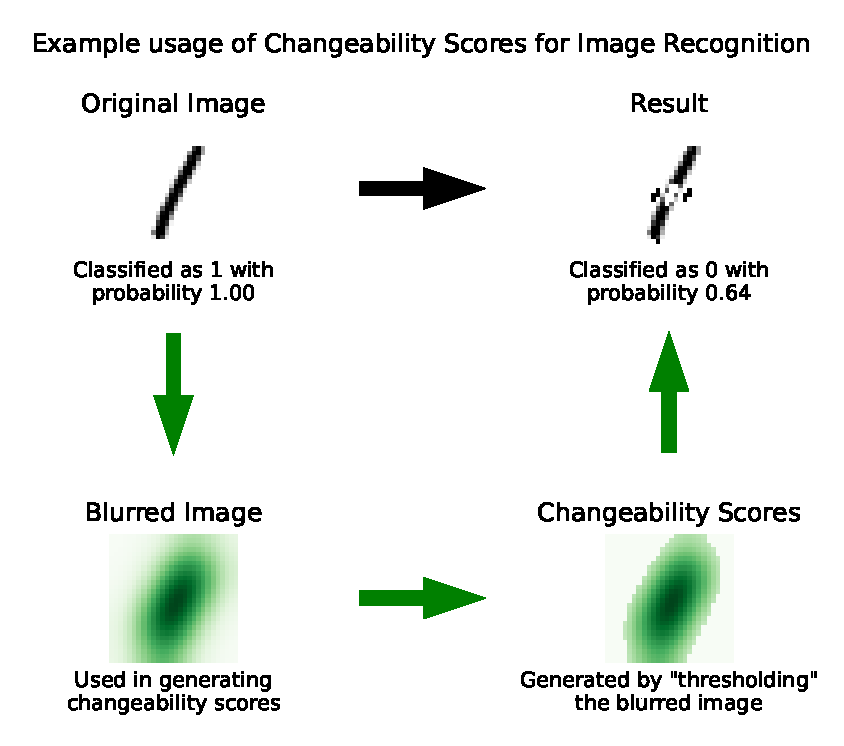
\includegraphics[width=\linewidth]{figures/mnist_changeability_example.eps}
    \caption{Example Example counterfactual generated with our proposed methodology. The first picture shows the original image, with the final showing the counterfactual. The middle images show some of the ``steps'' taken to get from the original image to the counterfactual.\label{figure:mnist_counterfactuals_changeability}}
\end{figure}

\subsection{Quantitative Evaluations}
Figures~\ref{figure:feature_changes} and~\ref{figure:distance} contains violin plots\footnote{Violin plots are similar to box plots, but also show the distribution of the data} of the various quantitative metrics defined in Section~\ref{section:evaluation_metrics}.

As shown in these figures, compared to comparable methods, our proposed methodology changes fewer features, but changes them by a larger amount (both in terms of \(L_1\) and \(L_2\) distance). In a sense, the counterfactuals are ``more interpretable'' as they change fewer features.

\begin{figure}
    \centering
    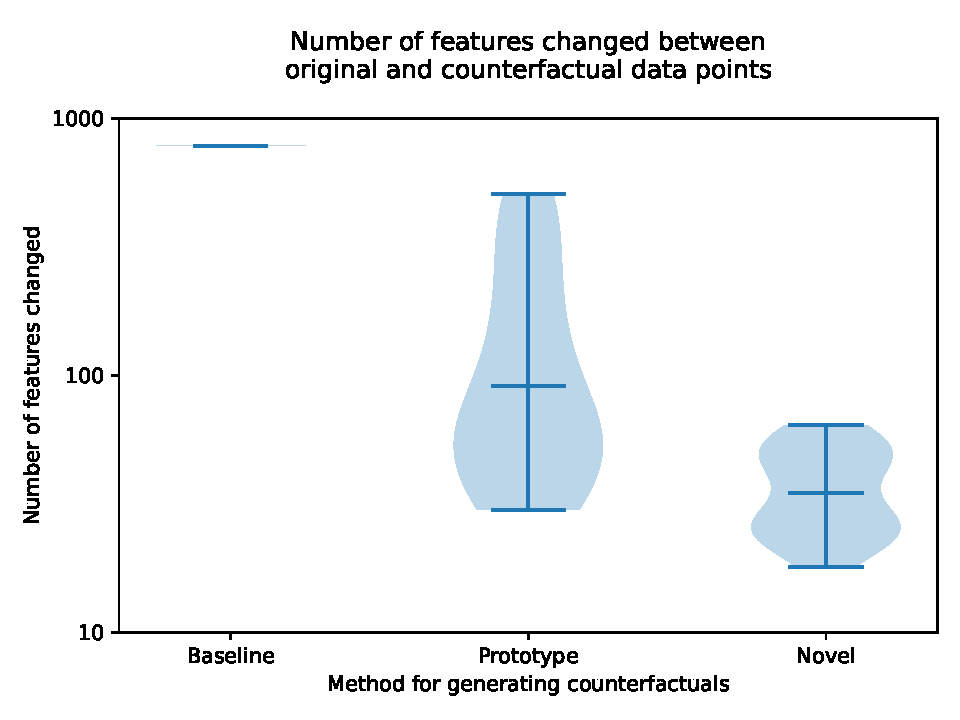
\includegraphics[width=\linewidth]{figures/counterfactual_features_changed.pdf}
    \caption{Violin plots of the number of feature changes for each method. The ``traditional'' method is that of~\cite{wachter_counterfactual_2017}, while the ``prototype'' method is that of~\cite{van_looveren_conditional_2021}.\label{figure:feature_changes}}
\end{figure}

\begin{figure}
    \centering
    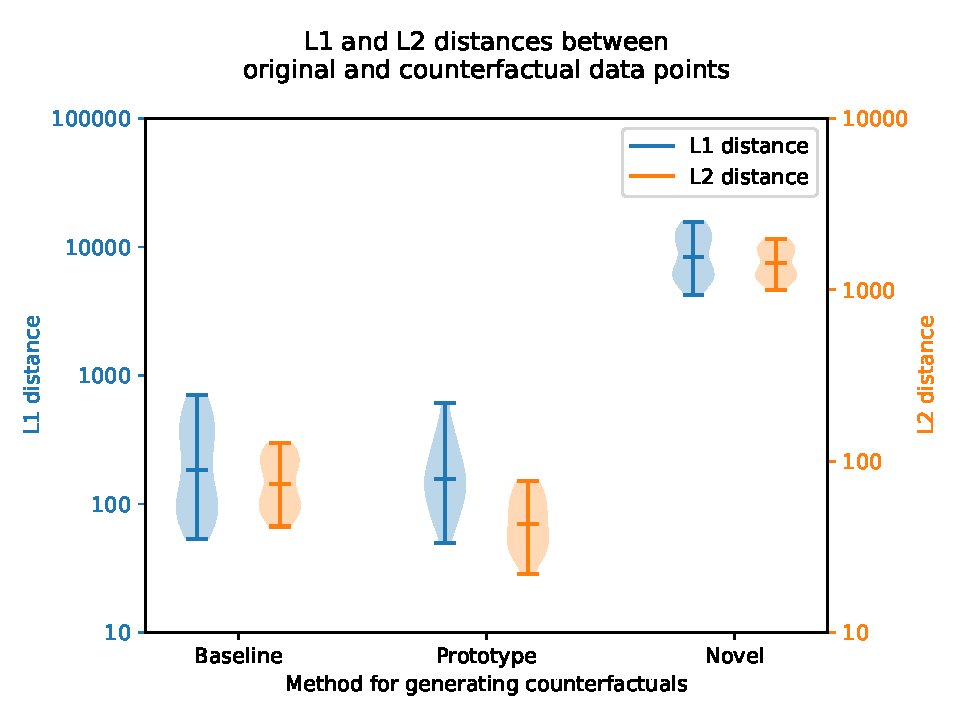
\includegraphics[width=\linewidth]{figures/counterfactual_distances.pdf}
    \caption{Violin plots of the \(L_1\) and \(L_2\) distances to the original data point for each method. The ``traditional'' method is that of~\cite{wachter_counterfactual_2017}, while the ``prototype'' method is that of~\cite{van_looveren_conditional_2021}.\label{figure:distance}}
\end{figure}

\section{Conclusions}
\subsection{Key Contributions}
In the project, we proposed a modular methodology to generate counterfactuals to explain black box models. This method borrows ideas from Human-Computer Interaction (HCI) research to develop a ``tuneable'', ``human-in-the-loop'' explanation method for machine learning models. We evaluated the model's performance on a range of data sets and examined variations of our method.

\bibliography{ref}

\end{document}
